\documentclass[tikz,border=5pt]{standalone}
\usepackage[utf8]{inputenc}
\usepackage[T1]{fontenc}
\usepackage{lmodern,amsmath,amssymb}
\usepackage[american]{circuitikz}
\usepackage{pgfplots}
\pgfplotsset{compat=1.18}
\usetikzlibrary{circuits.logic.US,positioning,calc,arrows.meta,patterns,shapes.geometric}
\definecolor{Primary}{HTML}{1F77B4}
\begin{document}
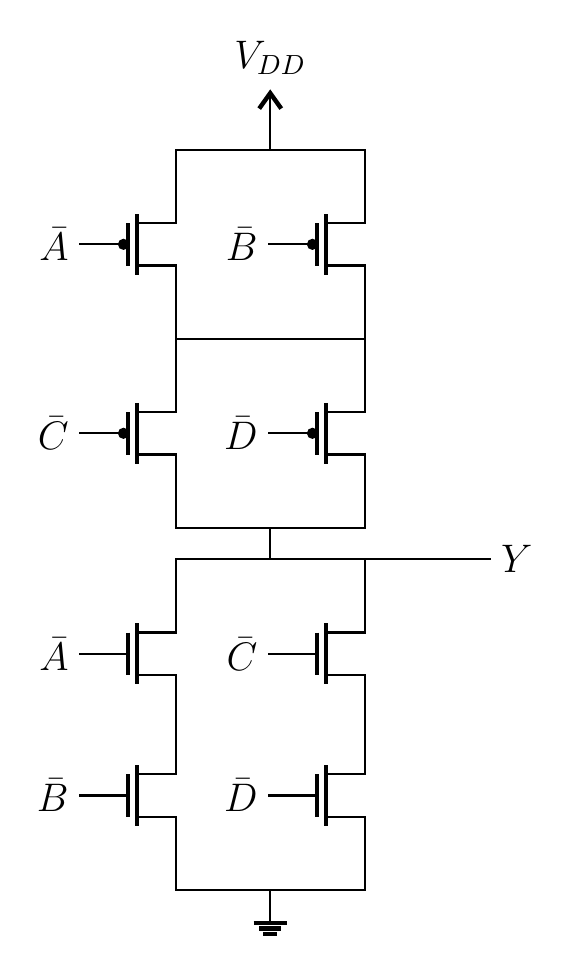
\begin{tikzpicture}[thick,font=\Large]\draw(0,5.2)--(-1.2,5.2)--(-1.2,4.9);\node[pmos](m5)at(-1.2,4.0){};\draw(-1.2,4.9)--(m5.S)(m5.D)--(-1.2,3.1000000000000005);\draw(m5.G)--++(-.25,0)node[left]{$\bar A$};\draw(-1.2,3.1000000000000005)--(-1.2,2.8000000000000003)--(0,2.8000000000000003);\draw(0,5.2)--(1.2,5.2)--(1.2,4.9);\node[pmos](m6)at(1.2,4.0){};\draw(1.2,4.9)--(m6.S)(m6.D)--(1.2,3.1000000000000005);\draw(m6.G)--++(-.25,0)node[left]{$\bar B$};\draw(1.2,3.1000000000000005)--(1.2,2.8000000000000003)--(0,2.8000000000000003);\draw(0,2.8000000000000003)--(-1.2,2.8000000000000003)--(-1.2,2.5000000000000004);\node[pmos](m7)at(-1.2,1.6000000000000005){};\draw(-1.2,2.5000000000000004)--(m7.S)(m7.D)--(-1.2,0.7000000000000004);\draw(m7.G)--++(-.25,0)node[left]{$\bar C$};\draw(-1.2,0.7000000000000004)--(-1.2,0.40000000000000036)--(0,0.40000000000000036);\draw(0,2.8000000000000003)--(1.2,2.8000000000000003)--(1.2,2.5000000000000004);\node[pmos](m8)at(1.2,1.6000000000000005){};\draw(1.2,2.5000000000000004)--(m8.S)(m8.D)--(1.2,0.7000000000000004);\draw(m8.G)--++(-.25,0)node[left]{$\bar D$};\draw(1.2,0.7000000000000004)--(1.2,0.40000000000000036)--(0,0.40000000000000036);\draw(0,0)--(-1.2,0)--(-1.2,-0.3);\node[nmos](m9)at(-1.2,-1.2){};\draw(-1.2,-0.3)--(m9.D)(m9.S)--(-1.2,-2.1);\draw(m9.G)--++(-.25,0)node[left]{$\bar A$};\node[nmos](m10)at(-1.2,-3.0){};\draw(-1.2,-2.1)--(m10.D)(m10.S)--(-1.2,-3.9000000000000004);\draw(m10.G)--++(-.25,0)node[left]{$\bar B$};\draw(-1.2,-3.9)--(-1.2,-4.2)--(0,-4.2);\draw(0,0)--(1.2,0)--(1.2,-0.3);\node[nmos](m11)at(1.2,-1.2){};\draw(1.2,-0.3)--(m11.D)(m11.S)--(1.2,-2.1);\draw(m11.G)--++(-.25,0)node[left]{$\bar C$};\node[nmos](m12)at(1.2,-3.0){};\draw(1.2,-2.1)--(m12.D)(m12.S)--(1.2,-3.9000000000000004);\draw(m12.G)--++(-.25,0)node[left]{$\bar D$};\draw(1.2,-3.9)--(1.2,-4.2)--(0,-4.2);\draw(0,5.2)--++(0,.3)node[vcc]{$V_{DD}$};\draw(0,.4)--(0,0)--(2.8,0)node[right]{$Y$};\draw(0,-4.2)node[ground]{};\end{tikzpicture}
\end{document}
